\begin{pastexam}[label={px:ntu-110-ie-ds-18}]{臺大工工所 110 學年度 第 18 題}
（複選；每題 5 分，每答錯一個選項倒扣 1 分至該題 0 分止）

In this exam, the height of a leaf (in either a tree or heap) is defined as 0; the depth of the root (in
either a tree or heap) is defined as 0.

Consider an AVL tree that results from successively inserting keys 2, 4, 5, 3, 8, 7, 1, 6, 9 into an
initially empty tree. Which of the following statements are true?
\begin{enumerate}[label=(\Alph*)]
\item The tree height is 4.
\item Key 3 and key 5 have the same depth.
\item Key 2 and key 8 have the same height.
\item Key 6 is a leaf.
\item Key 7 is the parent of key 9.
\end{enumerate}
\end{pastexam}

\begin{pastsoln}
答案是 (B)、(C)、(D)。

照資結書第~10.2.3~節的 AVL 插入逐一追蹤（只在失衡時旋轉）：
\begin{enumerate}
\item 插入 $2$、$4$：$2$ 為根，$4$ 是右子節點。
\item 插入 $5$：放在 $4$ 的右邊，$2$ 的平衡因子變成 $-2$，右右（RR）型，對 $2$ 左旋，$4$ 成為根，左 $2$、右 $5$。
\item 插入 $3$：放在 $2$ 的右邊，沒有失衡。
\item 插入 $8$：放在 $5$ 的右邊，沒有失衡（根的左右子樹高度都是 $1$）。
\item 插入 $7$：路徑 $4 \to 5 \to 8$，放在 $8$ 的左邊。 $5$ 的右子樹高 $1$、左子樹空，失衡，右左（RL）型：先對 $8$ 右旋、再對
$5$ 左旋，$7$ 升上來，左 $5$、右 $8$。
\item 插入 $1$：放在 $2$ 的左邊，沒有失衡。
\item 插入 $6$：路徑 $4 \to 7 \to 5$，放在 $5$ 的右邊。 $5$、$7$、$4$ 的平衡因子分別是 $-1$、$1$、$-1$，沒有失衡。
\item 插入 $9$：放在 $8$ 的右邊，沒有失衡。
\end{enumerate}
\begin{center}
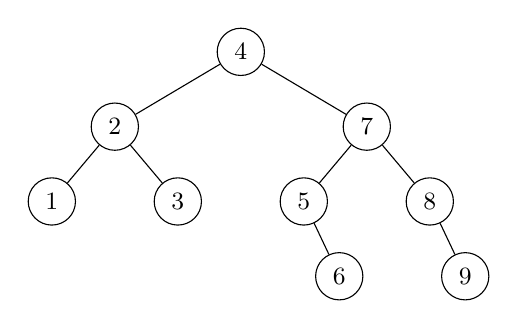
\begin{tikzpicture}[level distance=0.95cm,level 1/.style={sibling distance=3.2cm},
  level 2/.style={sibling distance=1.6cm},level 3/.style={sibling distance=0.9cm},
  every node/.style={circle,draw,minimum size=6mm,inner sep=0pt,font=\small}]
\node {4}
  child {node {2} child {node {1}} child {node {3}}}
  child {node {7}
    child {node {5} child[missing] child {node {6}}}
    child {node {8} child[missing] child {node {9}}}};
\end{tikzpicture}
\end{center}
各節點的高度（葉節點為 $0$）：$1, 3, 6, 9$ 是 $0$；$2, 5, 8$ 是 $1$；$7$ 是 $2$；根 $4$ 是 $3$。 深度：$4$ 是 $0$；
$2, 7$ 是 $1$；$1, 3, 5, 8$ 是 $2$；$6, 9$ 是 $3$。
\begin{itemize}
\item (A) 錯。 樹高是 $3$（例如 $4 \to 7 \to 5 \to 6$）。
\item (B) 對。 $3$、$5$ 的深度都是 $2$。
\item (C) 對。 $2$、$8$ 的高度都是 $1$。
\item (D) 對。 $6$ 是 $5$ 的右子節點，沒有子節點。
\item (E) 錯。 $9$ 的父節點是 $8$；$7$ 的子節點是 $5$ 和 $8$。
\end{itemize}
\end{pastsoln}
